%%%%%%%%%%%%%%%%%%%%%%%%%%%%%%%%%%%%%%%%%%%%%%%%%%%%%%%%%%%%%%%%%%
%%This presentation was fullly copied from the WSC presentation (dec. 2015)
%% and addapted for the CAA2k16
\documentclass[12pt, notes=show]{beamer}
\usetheme[width=0cm]{Goettingen}
\usecolortheme{rose}
\useoutertheme{default}
\setbeamerfont{caption}{size=\scriptsize}
\setbeamertemplate{navigation symbols}{}

\addtobeamertemplate{navigation symbols}{}{%
	\usebeamerfont{footline}%
	\usebeamercolor[fg]{footline}%
	\hspace{1em}%
	$\dfrac{\insertframenumber}{\inserttotalframenumber}$
}

\usepackage{hyperref}
\usepackage{fontspec} 
\setsansfont{Futura LT}
%\setmonofont[Scale=0.8]{Monaco} 


\usepackage{arydshln}

\usepackage{amsmath}

\usepackage{mathptmx}
\usepackage{latexsym}
\usepackage{mathtools}
\usepackage{multirow}
\usepackage{caption}
\usepackage{array}


\DeclarePairedDelimiter\abs{\lvert}{\rvert}%
\DeclarePairedDelimiter\norm{\lVert}{\rVert}%


\makeatletter
\let\oldabs\abs
\def\abs{\@ifstar{\oldabs}{\oldabs*}}
\let\oldnorm\norm
\def\norm{\@ifstar{\oldnorm}{\oldnorm*}}
\makeatother

\title{
	CAA2016\\
	Co-evolution of trade and culture\\
	Impact of cultural network topology on economic dynamics.
}

\institute{31 March 2016}

\author{Simon Carrignon, Jean-Marc Montanier, Jérôme Michaud \& Xavier Rubio-Campillo}

\date{
	\scriptsize
	\begin{columns}
		\begin{column}{.3\textwidth}
			\begin{center}
				Barcelona Supercomputing Center	\\
				
\includegraphics[height=1cm]{images/bscLogo.jpg} \hspace{2cm}
			\end{center}
		\end{column}
		\begin{column}{.3\textwidth}
			\begin{center}
				Univ. Pompeu Fabra Complex System Lab.\\
				\includegraphics[height=1cm]{images/upfLogo.jpeg} %declare logo image with an alias here 
			\end{center}
		\end{column}
	\end{columns}

}
\begin{document}
\begin{frame}
	\maketitle

\end{frame}

\begin{frame}{Plan of the presentation}
	\begin{enumerate}
		\item Co-evolution of trade and culture
			\vfill
		\item The Model
			\vfill
		\item Cultural Network Topologies
			\vfill
	\end{enumerate}

\end{frame}

\section{Introduction}
\begin{frame}{Cultural Evolution}
	\begin{center}
		\includegraphics[width=.4\textwidth]{images/beardevo.jpg} 
	\end{center}
	How Social Traits Evolve?
\end{frame}

\begin{frame}{Cultural Evolution}
	\begin{center}
		\includegraphics[width=4cm]{images/dalmatian.jpg} \hspace{2cm}
		\includegraphics[width=2cm]{images/pottery.jpg}\\
		\vspace{1cm}
		\includegraphics[width=4cm]{images/name.jpg}
	\end{center}
	%Similar variants distributions
	%\begin{figure}
	%	\begin{columns}
	%		\begin{column}{.8\textwidth}
	%			\centering
	%			\includegraphics[width=.6\textwidth]{images/powerlawrepartition.jpg}
	%		\end{column}
	%		\begin{column}{.3\textwidth}
	%			\tiny
	%			Square: male names\\
	%			Circle: female names\\
	%			From Bentley et al,~2004.
	%		\end{column}
	%	\end{columns}
	%\end{figure}
\end{frame}

\begin{frame}{What Generate Those Cultural Changes?}
	Simple mechanisms (Bentley et al, 2004):
	\begin{itemize}
		\item Random Copy 
		\item Frequency biased (conformist/anti-conformist\dots)
		\item \dots
	\end{itemize}
	\begin{figure}
		\begin{columns}
			\begin{column}{.8\textwidth}
				\centering
				\includegraphics[width=.6\textwidth]{images/powerlawrepartition.jpg}
			\end{column}
			\begin{column}{.3\textwidth}
				\tiny
				Square: male names\\
				Circle: female names\\
				Dotted and plain lines: model result with different copy probabilities.\\
				From Bentley et al,~2004.
			\end{column}
		\end{columns}
	\end{figure}
\end{frame}

\section{Context}



\begin{frame}{Trade and Cultural Network}
		What happen when such mechanisms act on social traits impacting trade?
	\begin{columns}
		\begin{column}{.4\textwidth}
			\includegraphics[width=\textwidth]{images/obsidianFlint.jpg}	
		\end{column}
		\begin{column}{.5\textwidth}
			\small
			Traits $+$ artefacts with ``economic'' value (\emph{ie}  \textit{Context} or \textit{Content} Biased).
			\begin{itemize}
				\item ``Usefulness''
				\item popularity
				\item availability
				\item \dots
			\end{itemize}
		\end{column}
	\end{columns}
\end{frame}

%\begin{frame}
%	\begin{center}
%		What happen when such mechanisms act on social traits impacting economy?
%	\end{center}
%	\begin{columns}
%		\begin{column}{.3\textwidth}
%			\includegraphics[width=\textwidth]{images/bordeaux.jpg}	
%		\end{column}
%		\begin{column}{.2\textwidth}
%		\end{column}
%		\begin{column}{.3\textwidth}
%			\includegraphics[width=3cm]{images/napa}	
%		\end{column}
%	\end{columns}
%\end{frame}

\begin{frame}{Co-evolution of Trade and Culture}

	%How Simple Cultural Dynamics influence Economy That in turn will influence cultural dynamics.

	\begin{alertblock}{Interaction between Culture and Trade}
		\begin{center}
			Social Interactions transform Trade Mechanisms \\
			\begin{center}
				$  \scalebox{3}{\circlearrowright}$
			\end{center}
			Trade mechanisms change Social Interactions
		\end{center}
	\end{alertblock}


\end{frame}


\section{ABM Framework}

%\begin{frame}{A General Agent Based Framework }
%	\begin{center}
%		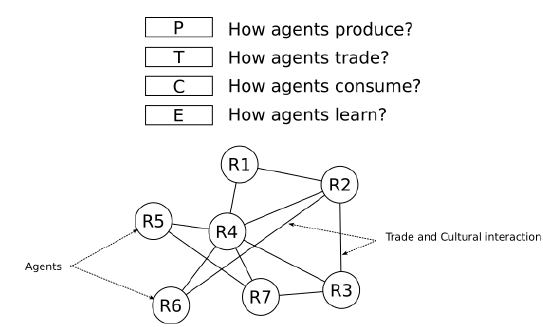
\includegraphics[width=.6\textwidth]{images/schema_model.png}
%	\end{center}
%\end{frame}



\begin{frame}{A General Agent Based Framework }

	Two main components:
	\vfill
	\begin{enumerate}
		\item Trade side: Bartering Economy (Gintis 2009),
			\vspace{1cm}
		\item Cultural side: ``copy the most successful'' (Bentley 2006).
	\end{enumerate}

	%How Simple Cultural Dynamics influence Economy That in turn will influence cultural dynamics.



\end{frame}

\begin{frame}{The Model}
	\begin{block}{1. The Economy \& the Barter Mechanism}
		\begin{itemize}
			\item $N$ goods
			\item $M$ Agent 
				$\left\{
					\begin{tabular}{@{}l@{}}
						a quantity of each Goods \\
						$N$ values attributed to each goods\\
					\end{tabular}
					\right.$
				\item Agents \emph{produce} one good and \emph{exchange} it to obtain the other goods.
				\item After the exchange, the agents \emph{consume} all goods 
			\end{itemize}

		\end{block}
	\end{frame}

	\begin{frame}{The Model}
		\begin{block}{2. Cultural Mechanisms}
			Every step:
			\begin{itemize}
				\item Economic activity (cf. previous slide).
				\item A \emph{score} is given following $f(q_n)$  a shared \& fixed ``utility function''.
			\end{itemize}
			After 10 steps:
			\begin{itemize}
				\item Less successful agents \emph{copy} the most successful (Biased-Copy).
				\item Given a probability $\mu$ the value attributed to some goods is modified (Innovation/Mutation)
			\end{itemize}
		\end{block}
	\end{frame}

	\begin{frame}
		\begin{center}
			\includegraphics[trim={2cm 6cm 2cm 5cm},clip,width=8cm]{images//trade-cultural.png}
		\end{center}
	\end{frame}

	\begin{frame}{The Model }
		\begin{figure}
			\caption{Example for 3 goods and 600 agents}
			\begin{columns}
				\column{.5\textwidth}
				\includegraphics[width=5cm]{images/full.pdf} 
							%\caption{Evolution of the score of the agents in a setup with 600 agents and 3 goods trading and exchanging their strategies during 10000 timesteps.}%%
			\end{columns}
			@~Equilibrium: mean of score  $\rightarrow$ score max.
		\end{figure}

	\end{frame}

	\section{Experimental Setup \& Results}
	\begin{frame}{Experiments}
		\textbf{Impact of the topology of the cultural network }
		\begin{center}
			``What properties of the cultural network influence the economic dynamics? '' 
		\end{center}
		\begin{center}
		\includegraphics[trim={2cm 6cm 2cm 5cm},clip,width=6cm]{images//trade-cultural2.png}
		\end{center}
		\vfil
		$\rightarrow$ Average Distance vs Average Degree\\




	\end{frame}


	\begin{frame}{Degree}
		\begin{center}
			\includegraphics<1>[height=.9\textheight]{images/smA.png} 	
			\includegraphics<2>[height=.9\textheight]{images/smAneighbours} 	
			\includegraphics<3>[height=.9\textheight]{images/smAk9.png} 	
		\end{center}
	\end{frame}
	\begin{frame}{Shortest Path Length}
		\begin{center}
			\includegraphics<1>[height=.9\textheight]{images/smA.png} 	
			\includegraphics<2>[height=.9\textheight]{images/smAB.png} 	
			\includegraphics<3>[height=.9\textheight]{images/smABlinked.png} 	
			\includegraphics<4>[height=.9\textheight]{images/smABlinkedL4.png} 	
		\end{center}
	\end{frame}
	\begin{frame}{Degree}
		\begin{center}
			\includegraphics<1>[height=.9\textheight]{images/hmA.png} 	
			\includegraphics<2>[height=.9\textheight]{images/hmAneighbours} 	
			\includegraphics<3>[height=.9\textheight]{images/hmAk4.png} 	
		\end{center}
	\end{frame}
	\begin{frame}{Shortest Path Length}
		\begin{center}
			\includegraphics<1>[height=.9\textheight]{images/hmA.png} 	
			\includegraphics<2>[height=.9\textheight]{images/hmAB.png} 	
			\includegraphics<3>[height=.9\textheight]{images/hmABlinked.png} 	
			\includegraphics<4>[height=.9\textheight]{images/hmABlinkedL25.png} 	
		\end{center}
	\end{frame}
%	\\Trade Mechanism + Success Biased Copy\\
%	\vfill
%	vs\\
%	\vfill
%	\textbf{Neutral Model}\\ Trade Mechanism + Random Copy\\

	\begin{frame}{Experimental Setup}
		Set of networks with combination of properties:
		\begin{itemize}
			\item Average Degree (D)
			\item Average Distance (A)
		\end{itemize}
		\begin{center}
			\begin{tabular}{l|ccc}
				& $\left\langle k \right\rangle_1$ & \dots & $\left\langle k \right\rangle_n$\\
				\hline\\
				$L_1$	& $G_{11}$	& 	& $G_{1n}$	\\	
				\dots	&		&\dots	&		\\
				$L_m$	& $G_{m1}$	& 	& $G_{mn}$	\\	
			\end{tabular}
		\end{center}

	\end{frame}
	\begin{frame}{Experimental Setup}
		\begin{table}
			\centering
			\begin{tabular}{m{1.2cm}m{2.5cm}m{2.5cm}}
				&$\left\langle k\right\rangle=8$ & $\left\langle k\right\rangle=4$\\
				$L\approx17$&
				\includegraphics[width=2.5cm]{images/g02.pdf}&
				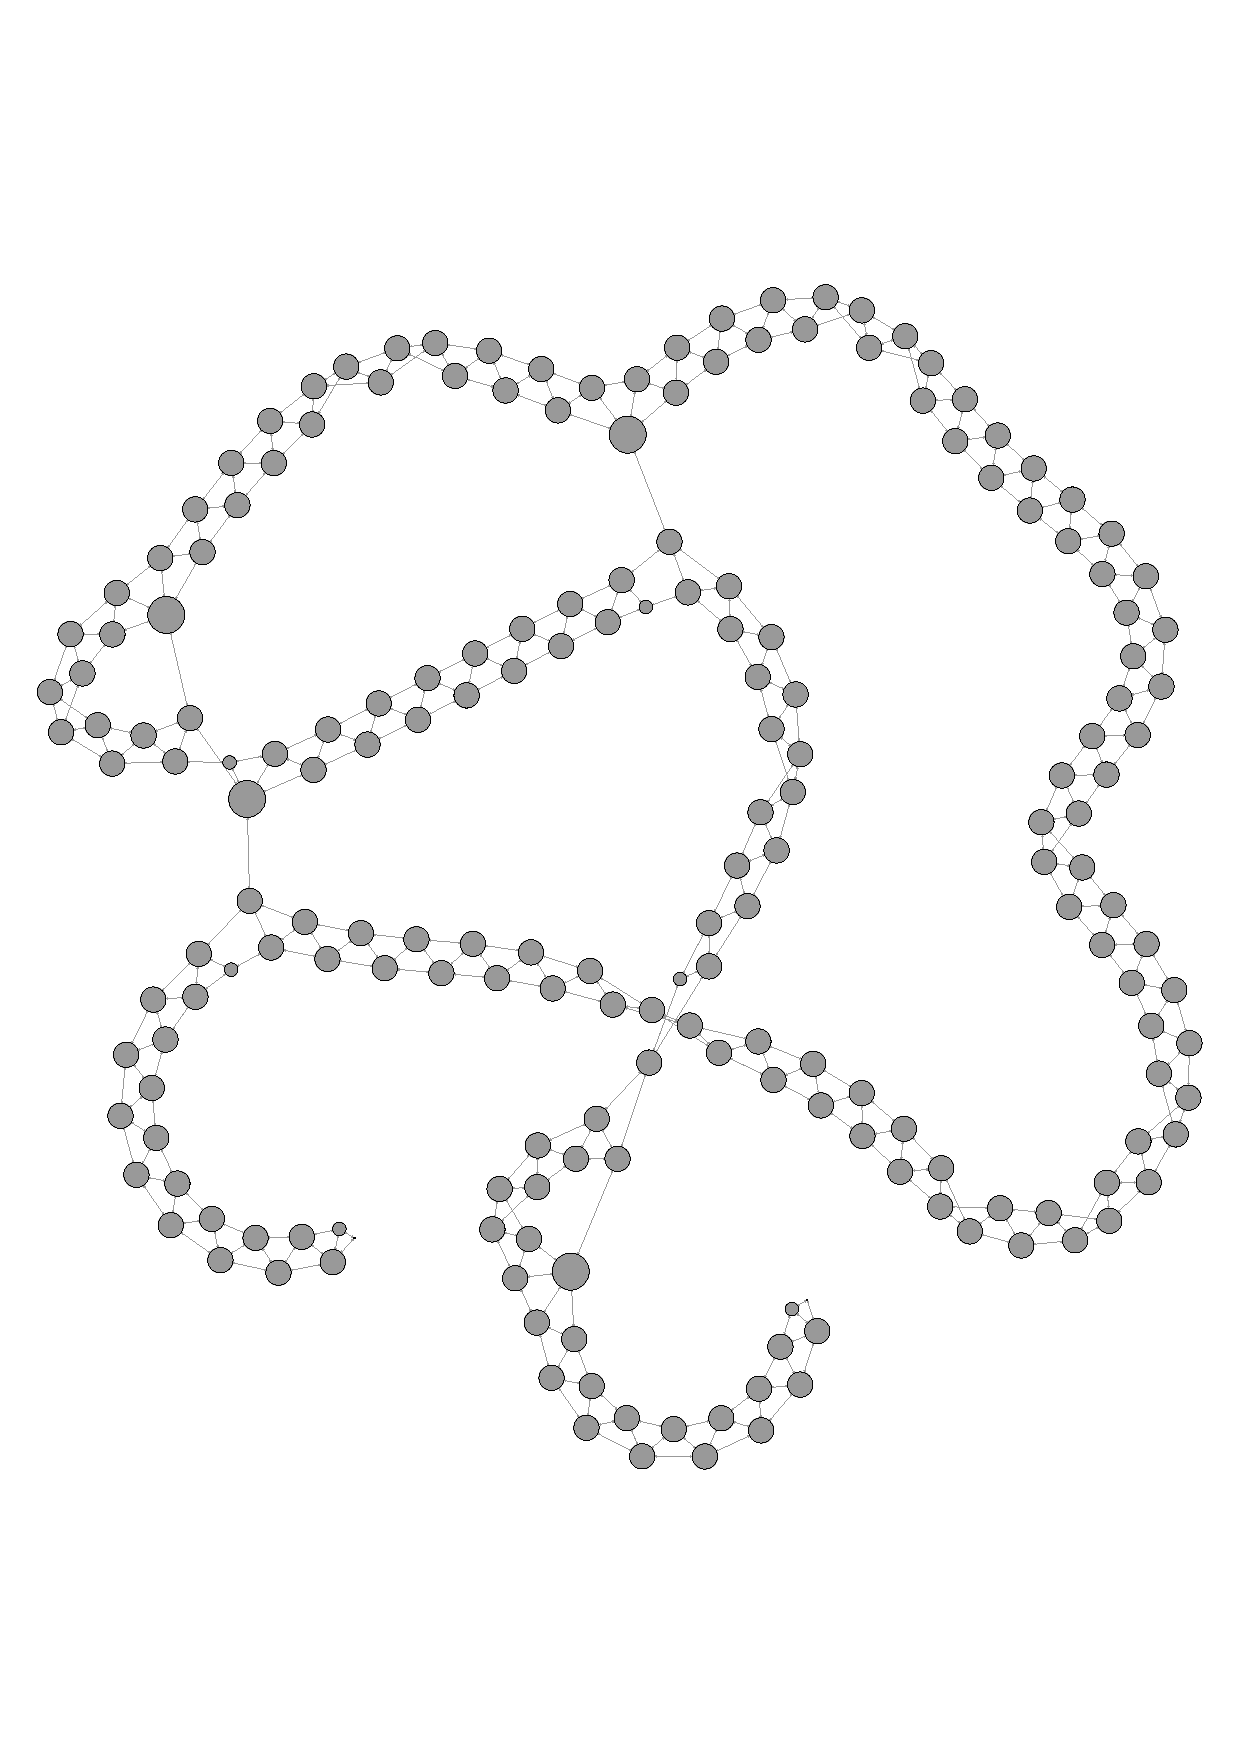
\includegraphics[width=2.5cm]{images/g00.pdf}\\
				$L\approx4$&
				\includegraphics[width=2.5cm]{images/g42.pdf}&
				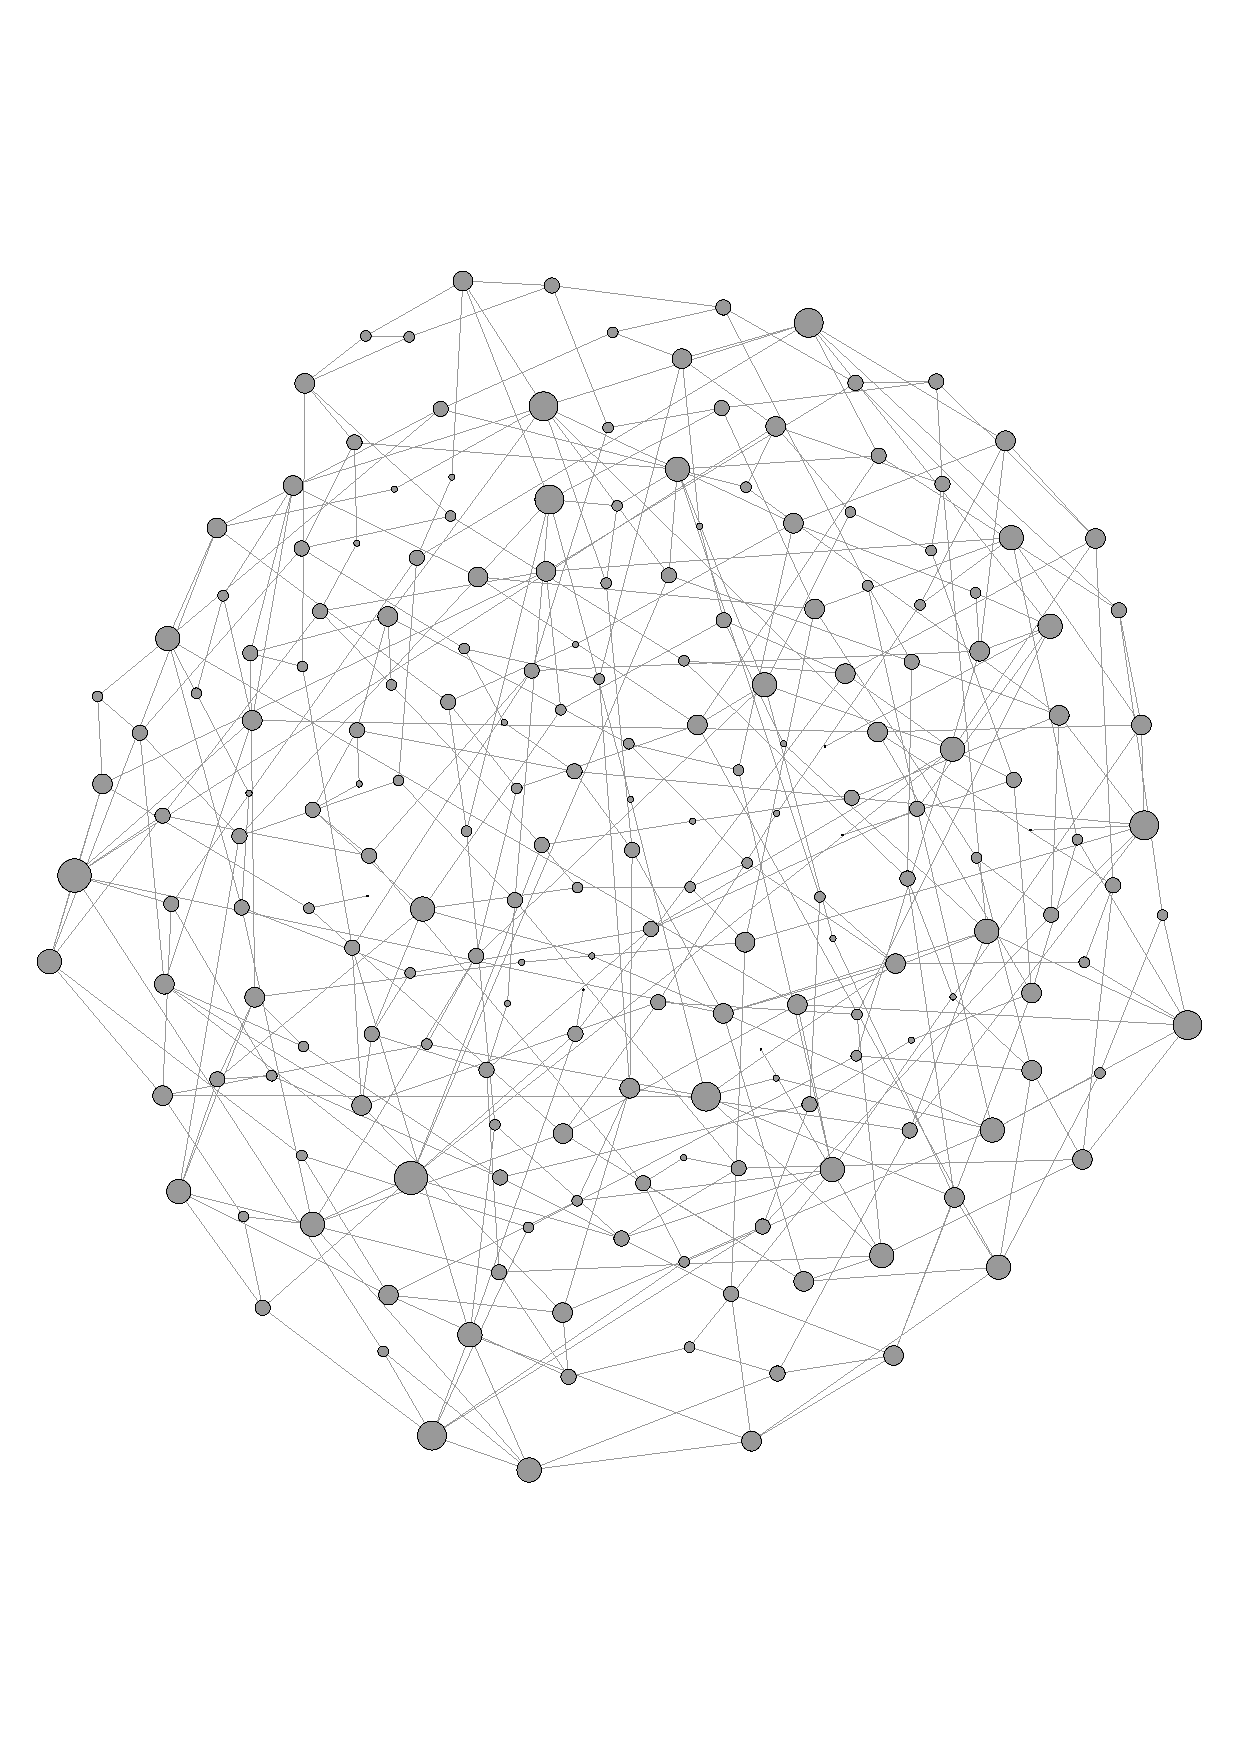
\includegraphics[width=2.5cm]{images/g40.pdf}\\
			\end{tabular}
		\end{table}
	\end{frame}



	\begin{frame}{Results: }
					General Behaviour of the simulations with different topologies.
		\begin{figure}[h]
			\begin{center}
						\includegraphics[height=.5\textheight]{images//provResults2.pdf}
			\end{center}
		\end{figure}

	\end{frame}

	\begin{frame}{Results: }
		\begin{figure}[h]

			Time of convergence as a function of $L$.
			\begin{center}
						%Behaviour of the simulations with different topologies.}
						\includegraphics[height=.6\textheight]{images//L_vs_t10.pdf}

			\end{center}
		\end{figure}

	\end{frame}




	\begin{frame}{Summary}
		\begin{itemize}
			\item Simple cultural mechanism can lead to efficient trade dynamics:\\
				{$\rightarrow$ \small Both aspect should be studied together.}
				\vfill
			\item Properties of the cultural network impact thoses dynamics.\\
				{$\rightarrow$\small Different network support different economy}
				\vfill
		\end{itemize}

	\end{frame}
	\begin{frame}{Future Works}
		
		\begin{enumerate}
			\item \emph{Non-equilibrium} conditions,
			\item Comparaison with ``real-world'' data,
			\item \dots
		\end{enumerate}
	\end{frame}

%\section{Application}
%\begin{frame}{Case Study}
%	Roman Empire Economy: \\
%	Tight link between economy and culture, trace of it. \\
%	\begin{figure}
%		\includegraphics[width=.6\textwidth]{images/dressel-filiation.jpg}
%	\end{figure}
%	
%\end{frame}
%
%\begin{frame}{Case Study}
%	Simulation as a tool to implement and test Historical Hypothesis.
%	\begin{itemize}
%	\item Network Constraints
%	\item Temporal Constraints
%	\item Different Cultural Mechanisms
%	\end{itemize}
%\end{frame}
	\begin{frame}{}
		\begin{center}
			\huge
			Thank for you attention!\\\vfill
			\includegraphics[width=2cm]{images/LOGO-ERC.jpg} \hfil	\includegraphics[width=3cm]{images/epnetLogo.png}\\
			\vspace{1cm}
			\scriptsize
			http://www.roman-ep.net/\\
			@epnetproject\\
			fb.com/EPNetProject\\
			@simoncarrignon
		\end{center}


	\end{frame}

	\end{document}


